\documentclass[14pt]{extbook}
\usepackage{multicol, enumerate, enumitem, hyperref, color, soul, setspace, parskip, fancyhdr} %General Packages
\usepackage{amssymb, amsthm, amsmath, bbm, latexsym, units, mathtools} %Math Packages
\everymath{\displaystyle} %All math in Display Style
% Packages with additional options
\usepackage[headsep=0.5cm,headheight=12pt, left=1 in,right= 1 in,top= 1 in,bottom= 1 in]{geometry}
\usepackage[usenames,dvipsnames]{xcolor}
\usepackage{dashrule}  % Package to use the command below to create lines between items
\newcommand{\litem}[1]{\item#1\hspace*{-1cm}\rule{\textwidth}{0.4pt}}
\pagestyle{fancy}
\lhead{Progress Quiz 9}
\chead{}
\rhead{Version B}
\lfoot{8590-6105}
\cfoot{}
\rfoot{Fall 2020}
\begin{document}

\begin{enumerate}
\litem{
Determine the vertical asymptotes and holes in the rational function below.\[ f(x) = \frac{4x^{3} +8 x^{2} -27 x -45}{6x^{2} -11 x -10} \]\begin{enumerate}[label=\Alph*.]
\item \( \text{Vertical Asymptotes of } x = -0.667 \text{ and } x = -1.5 \text{ with a hole at } x = 2.5 \)
\item \( \text{Vertical Asymptote of } x = 0.667 \text{ and hole at } x = 2.5 \)
\item \( \text{Holes at } x = -0.667 \text{ and } x = 2.5 \text{ with no vertical asymptotes.} \)
\item \( \text{Vertical Asymptote of } x = -0.667 \text{ and hole at } x = 2.5 \)
\item \( \text{Vertical Asymptotes of } x = -0.667 \text{ and } x = 2.5 \text{ with no holes.} \)

\end{enumerate} }
\litem{
Determine the horizontal and/or oblique asymptotes in the rational function below.\[ f(x) = \frac{10x^{3} -29 x^{2} +9 x + 18}{20x^{3} -1 x^{2} +11 x + 30} \]\begin{enumerate}[label=\Alph*.]
\item \( \text{Vertical Asymptote of } y = 2  \)
\item \( \text{Horizontal Asymptote of } y = 0.500  \)
\item \( \text{Horizontal Asymptote of } y = 0  \)
\item \( \text{None of the above} \)
\item \( \text{Vertical Asymptote of } y = 1.250  \)

\end{enumerate} }
\litem{
Determine the horizontal and/or oblique asymptotes in the rational function below.\[ f(x) = \frac{8x^{3} -22 x^{2} -5 x + 25}{4x^{2} +15 x -25} \]\begin{enumerate}[label=\Alph*.]
\item \( \text{Oblique Asymptote of } y = 2x -13. \)
\item \( \text{Horizontal Asymptote of } y = 2.0  \)
\item \( \text{Horizontal Asymptote of } y = 2.0 \text{ and Oblique Asymptote of } y = 2x -13 \)
\item \( \text{Horizontal Asymptote at } y = -5.0 \)
\item \( \text{Horizontal Asymptote of } y = -5.0 \text{ and Oblique Asymptote of } y = 2x -13 \)

\end{enumerate} }
\litem{
Determine the vertical asymptotes and holes in the rational function below.\[ f(x) = \frac{12x^{3} -29 x^{2} +23 x -6}{9x^{2} -18 x + 8} \]\begin{enumerate}[label=\Alph*.]
\item \( \text{Holes at } x = 1.333 \text{ and } x = 0.667 \text{ with no vertical asymptotes.} \)
\item \( \text{Vertical Asymptote of } x = 1.333 \text{ and hole at } x = 0.667 \)
\item \( \text{Vertical Asymptote of } x = 1.333 \text{ and hole at } x = 0.667 \)
\item \( \text{Vertical Asymptotes of } x = 1.333 \text{ and } x = 0.667 \text{ with no holes.} \)
\item \( \text{Vertical Asymptotes of } x = 1.333 \text{ and } x = 0.75 \text{ with a hole at } x = 0.667 \)

\end{enumerate} }
\litem{
Which of the following functions \textit{could} be the graph below?
\begin{center}
    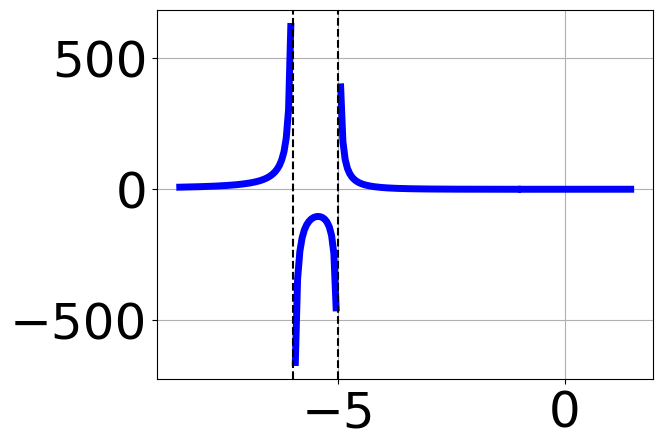
\includegraphics[width=0.5\textwidth]{../Figures/identifyGraphOfRationalFunctionB.png}
\end{center}
\begin{enumerate}[label=\Alph*.]
\item \( f(x)=\frac{x^{3} +5 x^{2} -9 x -45}{x^{3} +9 x^{2} +26 x + 24} \)
\item \( f(x)=\frac{x^{3} -7 x^{2} -5 x + 75}{x^{3} -9 x^{2} +26 x -24} \)
\item \( f(x)=\frac{x^{3} -5 x^{2} -9 x + 45}{x^{3} -9 x^{2} +26 x -24} \)
\item \( f(x)=\frac{x^{3} +5 x^{2} -9 x -45}{x^{3} +9 x^{2} +26 x + 24} \)
\item \( \text{None of the above are possible equations for the graph.} \)

\end{enumerate} }
\litem{
Determine the vertical asymptotes and holes in the rational function below.\[ f(x) = \frac{16x^{3} -24 x^{2} -31 x + 30}{12x^{2} -25 x + 12} \]\begin{enumerate}[label=\Alph*.]
\item \( \text{Vertical Asymptote of } x = 1.333 \text{ and hole at } x = 0.75 \)
\item \( \text{Vertical Asymptote of } x = 1.333 \text{ and hole at } x = 0.75 \)
\item \( \text{Holes at } x = 1.333 \text{ and } x = 0.75 \text{ with no vertical asymptotes.} \)
\item \( \text{Vertical Asymptotes of } x = 1.333 \text{ and } x = 0.75 \text{ with no holes.} \)
\item \( \text{Vertical Asymptotes of } x = 1.333 \text{ and } x = -1.25 \text{ with a hole at } x = 0.75 \)

\end{enumerate} }
\litem{
Determine the horizontal and/or oblique asymptotes in the rational function below.\[ f(x) = \frac{15x^{3} -82 x^{2} +131 x -60}{-20x^{3} +12 x^{2} +28 x -48} \]\begin{enumerate}[label=\Alph*.]
\item \( \text{Vertical Asymptote of } y = 3  \)
\item \( \text{None of the above} \)
\item \( \text{Vertical Asymptote of } y = -1.000  \)
\item \( \text{Horizontal Asymptote of } y = 0  \)
\item \( \text{Horizontal Asymptote of } y = -0.750  \)

\end{enumerate} }
\litem{
Determine the horizontal and/or oblique asymptotes in the rational function below.\[ f(x) = \frac{6x^{3} + x^{2} -30 x -25}{3x^{2} +20 x + 25} \]\begin{enumerate}[label=\Alph*.]
\item \( \text{Horizontal Asymptote of } y = 2.0  \)
\item \( \text{Horizontal Asymptote of } y = -5.0 \text{ and Oblique Asymptote of } y = 2x -13 \)
\item \( \text{Horizontal Asymptote at } y = -5.0 \)
\item \( \text{Horizontal Asymptote of } y = 2.0 \text{ and Oblique Asymptote of } y = 2x -13 \)
\item \( \text{Oblique Asymptote of } y = 2x -13. \)

\end{enumerate} }
\litem{
Determine the vertical asymptotes and holes in the rational function below.\[ f(x) = \frac{9x^{3} -12 x^{2} -20 x + 16}{12x^{2} +7 x -12} \]\begin{enumerate}[label=\Alph*.]
\item \( \text{Vertical Asymptotes of } x = 0.75 \text{ and } x = 0.667 \text{ with a hole at } x = -1.333 \)
\item \( \text{Vertical Asymptote of } x = 0.75 \text{ and hole at } x = -1.333 \)
\item \( \text{Holes at } x = 0.75 \text{ and } x = -1.333 \text{ with no vertical asymptotes.} \)
\item \( \text{Vertical Asymptotes of } x = 0.75 \text{ and } x = -1.333 \text{ with no holes.} \)
\item \( \text{Vertical Asymptote of } x = 0.75 \text{ and hole at } x = -1.333 \)

\end{enumerate} }
\litem{
Which of the following functions \textit{could} be the graph below?
\begin{center}
    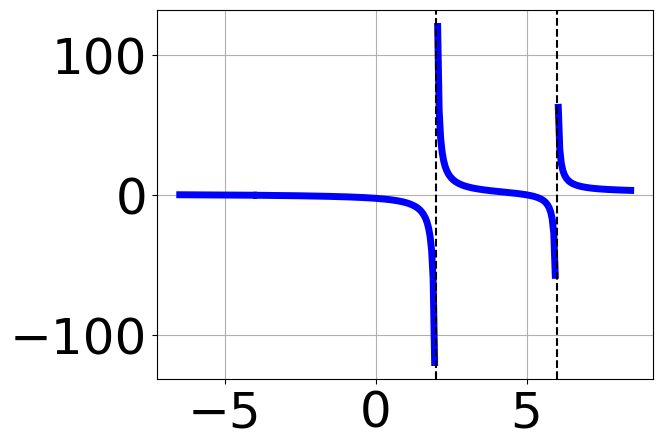
\includegraphics[width=0.5\textwidth]{../Figures/identifyGraphOfRationalFunctionCopyB.png}
\end{center}
\begin{enumerate}[label=\Alph*.]
\item \( f(x)=\frac{x^{3} +8 x^{2} -23 x -210}{x^{3} -4 x^{2} -20 x + 48} \)
\item \( f(x)=\frac{x^{3} -5 x^{2} -26 x + 120}{x^{3} +4 x^{2} -20 x -48} \)
\item \( f(x)=\frac{x^{3} +5 x^{2} -26 x -120}{x^{3} -4 x^{2} -20 x + 48} \)
\item \( f(x)=\frac{x^{3} -5 x^{2} -26 x + 120}{x^{3} +4 x^{2} -20 x -48} \)
\item \( \text{None of the above are possible equations for the graph.} \)

\end{enumerate} }
\end{enumerate}

\end{document}